\let\negmedspace\undefined
\let\negthickspace\undefined
\documentclass[journal]{IEEEtran}
\usepackage[a4paper, margin=10mm, onecolumn]{geometry}
%\usepackage{lmodern} % Ensure lmodern is loaded for pdflatex
\usepackage{tfrupee} % Include tfrupee package

\setlength{\headheight}{1cm} % Set the height of the header box
\setlength{\headsep}{0mm}  % Set the distance between the header box and the top of the text

\usepackage{gvv-book}
\usepackage{gvv}
\usepackage{cite}
\usepackage{amsmath,amssymb,amsfonts,amsthm}
\usepackage{algorithmic}
\usepackage{graphicx}
\usepackage{float}
\usepackage{textcomp}
\usepackage{xcolor}
\usepackage{txfonts}
\usepackage{listings}
\usepackage{enumitem}
\usepackage{mathtools}
\usepackage{gensymb}
\usepackage{comment}
\usepackage[breaklinks=true]{hyperref}
\usepackage{tkz-euclide} 
\usepackage{listings}
% \usepackage{gvv}                                        
\def\inputGnumericTable{}                                 
\usepackage[latin1]{inputenc}                                
\usepackage{color}                                            
\usepackage{array}                                            
\usepackage{longtable}                                       
\usepackage{calc}                                             
\usepackage{multirow}                                         
\usepackage{hhline}                                           
\usepackage{ifthen}                                           
\usepackage{lscape}
\usepackage{tikz}
\usetikzlibrary{patterns}

\begin{document}

\bibliographystyle{IEEEtran}
\vspace{3cm}

\title{12.492}
\author{ee25btech11063-vejith}

\maketitle
% \maketitle
% \newpage
% \bigskip
{\let\newpage\relax\maketitle}
\renewcommand{\thefigure}{\theenumi}
\renewcommand{\thetable}{\theenumi}
\setlength{\intextsep}{10pt} % Space between text and floats
\textbf{Question}:\\
Direction cosines of the vector $3\vec{\hat{i}} + -2\vec{\hat{j}} + 6\vec{\hat{k}}$ are
\begin{enumerate}[label=\alph*)]
    \begin{multicols}{2}
        \item \sbrak{3/7,-2/7,6/7}
        \item \sbrak{-3/7,2/7,-6/7}
       \item \sbrak{-7/3,7/2,-7/6}
        \item \sbrak{7/3,-7/2,7/6}
    \end{multicols}
\end{enumerate}
\textbf{Solution}:\\
let 
\begin{align}
    \Vec{r} = \myvec{3\\-2\\6}\\
    \norm{\vec{r}}=\sqrt{9 +4 +36}\\
\implies \norm{\vec{r}}=7
\end{align}
The unit  vector in the direction of $\vec{r}$  is
\begin{align}
    \frac{\vec{r}}{\norm{\vec{r}}} &= \frac{1}{7}\myvec{3\\-2\\6} = \myvec{\frac{3}{7}\\\frac{-2}{7}\\\frac{6}{7}}
    \end{align}

    \begin{figure}[h!]
   \centering
   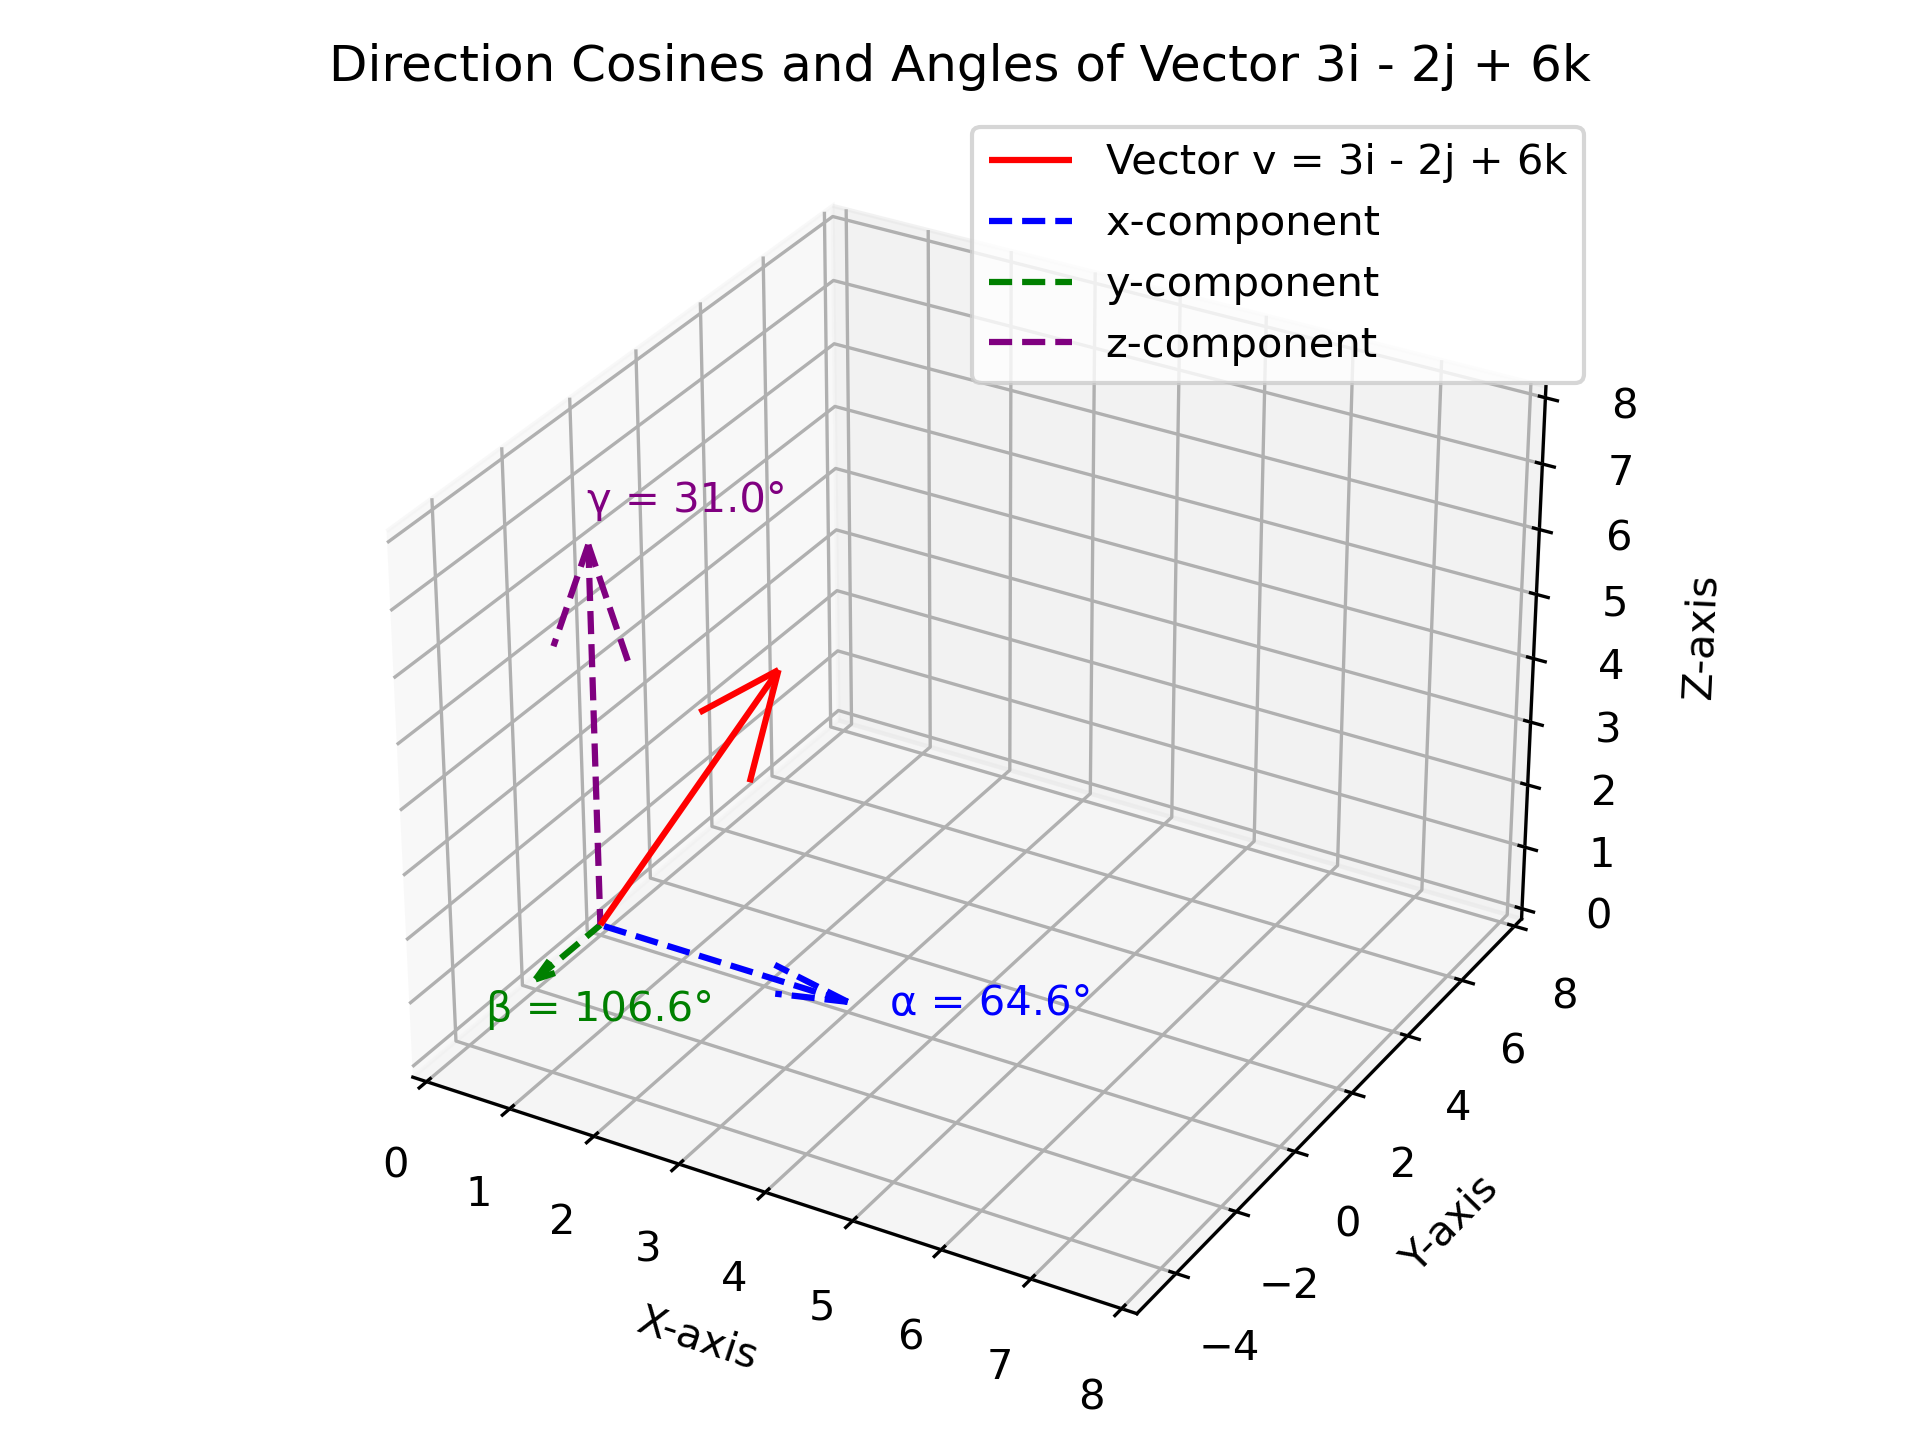
\includegraphics[width=0.8\columnwidth]{figs/01.png}
   \caption{}
   \label{}
\end{figure}
\end{document}
